\subsection{GAN Mel-Spectrogram Results}
We trained this form of the GAN to construct 64x64 Mel-Spectrogram images from noise. We used two popular models for ConvNet image generation for the generator/discriminator architecture:
\begin{itemize}
\item \textit{DCGAN} \cite{radford2015unsupervised} models the generator as a series of deconvolutional layers with ReLU activations, and the discriminator as a series of convolutional ones with leaky ReLU activations. Both architectures use batch normalization after each layer.
\item \textit{ResNet} \cite{ledig2016photo} GAN models the generator and discriminator each as very deep convnets (30 layers in our experiments) with upsampling/downsampling respectively. Residual (skip) connections are added every few layers to make training easier.
\end{itemize}
Visual results are demonstrated below. We generally used the same parameters as the \cite{gulrajani2017improved} paper, namely 5 critic iterations per generator iteration, a gradient penalty weight of 10, and batch size of 64. We saw recognizable spectrogram-like features in the data after only 1000 generator iterations, and after 5000 the generated samples were indistinguishable from real ones. Training took around 10 hours for 20000 iterations on a single 4 GB Nvidia GK104GL GPU.
\begin{figure}[h]
    \centering
    \begin{subfigure}[b]{0.4\textwidth}
        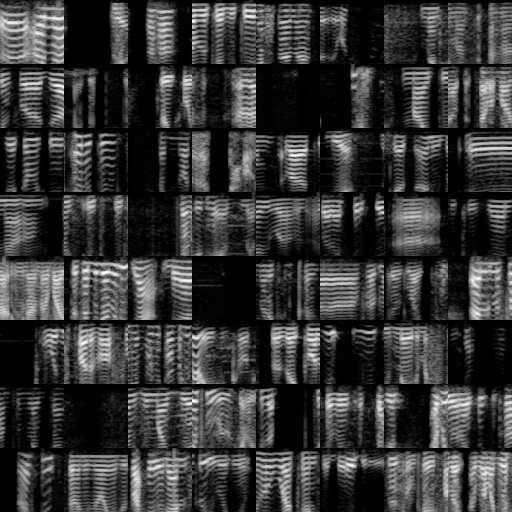
\includegraphics[width=\textwidth]{./fig/samples_groundtruth.png}
        \caption{Actual}
        \label{fig:samples_real}
    \end{subfigure}
    \qquad
    \begin{subfigure}[b]{0.4\textwidth}
        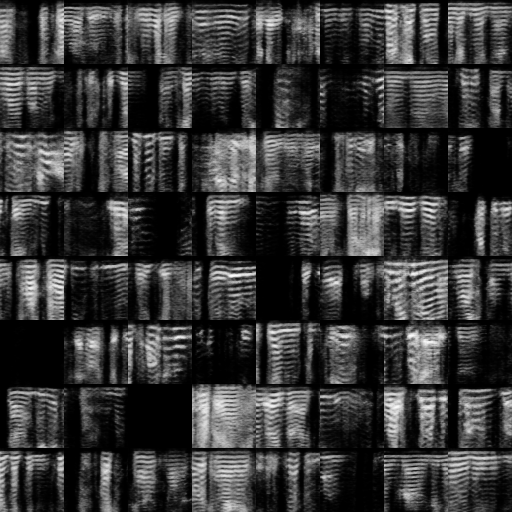
\includegraphics[width=\textwidth]{./fig/samples_5419.png}
        \caption{Generated}
        \label{fig:samples_fake}
    \end{subfigure}
    \caption{Comparison of real and generated ($\sim$ 5000 generator iterations) spectrogram samples. Each grid contains 64 samples.}
    \label{fig:samples_comparison}
\end{figure}

\subsection{Adversarial attacks}

Within the GAN framework, untargeted models are trained by using all data available, irrespective of class label. We show that an untargeted model able to generate data from the real distribution of the data and with enough variety can be used to perform adversarial attacks by classifying the samples produced by the generator. We provide details in the Untargeted attacks subsection.
The models for targeted attacks can be trained in two manners. The first is based on conditioning the model on additional information, e.g. class labels, as described in~\cite{mirza2014conditional}. The second is based on using only data from the label of interest. A drawback of the second approach is that the discriminator, and by consequence the generator, does not have access to universal\footnote{We draw a parallel with Universal Background Models in speech}. properties of speech. To circumvent this problem, we propose a new objective function that allows using the data from all classes, although the generator is learning how to generate one class. 

\subsubsection{Untargeted attacks}

For each of the speech in test set, we use the Mel-Spectrogram algorithm in section \ref{sub:processdata} to transform them into Mel-Spectrograms. The resulting mel-spectrogram is then fed into the CNN verifier and we extract a 505-dimensional feature $G$ from the penultimate fully-connected layer (L7) in the pre-trained CNN model (\ref{fig:CNN}) trained on the real speech dataset with all speaker ID. The deep feature $G$ is then used to train a K-nearest-neighbor (KNN) classifier.

To control the generator trained by our WGAN, we feed the generated Mel-Spectrograms into the same CNN-L2 pipeline to extract their corresponding feature $\widehat G$. Utilizing the pre-trained KNN, each sample is assigned to the nearest speaker in the deep feature space. Therefore, we know which speaker our generated sample belongs to when we attack our CNN verifier. We evaluate our controlled WGAN samples against the state-of-the-art CNN verifier, and the confusion matrix can be found in Figure \ref{fig:conf_mat_cnn_knn}. Although not included in the figure, \textbf{neither WaveNet samples nor SampleRNN samples were able to attack the recognition model in the same way.} \footnote{We also use the old state-of-the-art GMM-UBM speaker verifier.}


\begin{figure}[t]
    \centering
    \begin{subfigure}[b]{0.4\textwidth}
        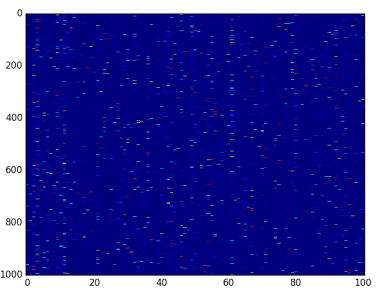
\includegraphics[width=\textwidth]{./fig/conf_mat_untargeted.png}
        \caption{activation of fully-connected layer (L2) on randomly sampled speech}
        \label{fig:yoyo_untargeted}
    \end{subfigure}
    \qquad
    \begin{subfigure}[b]{0.4\textwidth}
        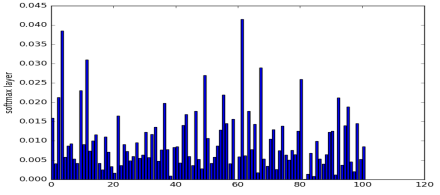
\includegraphics[width=\textwidth]{./fig/histogram_untargeted.png}
        \caption{distribution of randomly sampled speech from the generative model}
        \label{fig:histogram_untargeted}
    \end{subfigure}
    \caption{Summary of Untargeted Attacks}
    \label{fig:histogram_summary}
\end{figure}

Figure \ref{fig:histogram_untargeted} depicts that our GAN-trained generator successfully learns all speakers across the dataset, without mode collapsing.

\subsubsection{Targeted attacks}
However, the most natural attack is one in which we train a GAN to directly fool a speaker-authentication system, i.e., to produce samples that the system classifies as matching a target speaker with reasonable confidence. To train our WGAN in this way, we propose a modification to the critic that allows it to learn differentiate between not only real samples and generated samples, but also between real speech samples from a target speaker and real speech samples from other speakers. We do this by adding a term to the critic's loss that encourages its discriminator to classify real speech samples from untargeted speakers as fake. The critic's loss $L_C$ becomes:
\begin{align}
    \underbrace{\underset{\boldsymbol{\widetilde{x}} \sim \mathbb{P}_{g}}{\mathbb{E}}  \big[D(\boldsymbol{\widetilde{x}})\big]}_\text{Generated Samples} \color{red} + \alpha * \underbrace{\underset{\boldsymbol{\dot{x}} \sim \mathbb{P}_{\dot{x}}}{\mathbb{E}}  \big[D(\boldsymbol{\dot{x}})\big]}_\text{Different Speakers} \color{black} - \underbrace{\underset{\boldsymbol{x} \sim \mathbb{P}_{r}}{\mathbb{E}}  \big[D(\boldsymbol{x})\big]}_\text{Real Speaker}  + \underbrace{\lambda \underset{\boldsymbol{\hat{x}} \sim \mathbb{P}_{\hat{x}}}{\mathbb{E}}  \big[(\lVert \nabla_{\boldsymbol{\hat{x}}} D(\boldsymbol{\hat{x}}) \rVert_2 - 1)^2\big]}_\text{Gradient Penalty}
\end{align}
where $P_{\hat{x}}$ is the distribution of samples from other speakers, and $\alpha$ is a tunable scaling factor. In our experiments, we trained this GAN with 1 target speaker and a set of 99 'other' speakers. On each of the critic, we would feed the critic a batch of samples from one target speaker, and a batch of data uniformly sampled from the other speakers. We used an $\alpha$ of 0.1 (we found that not including this scaling factor led to serious the critic seriously overfitting and poor convergence of the GAN). Results are demonstrated in figure 4 b): The confusion  matrix demonstrates all energy is concentrated in speaker id 2. 
\begin{figure}[t]
    \centering
    \begin{subfigure}[b]{0.4\textwidth}
        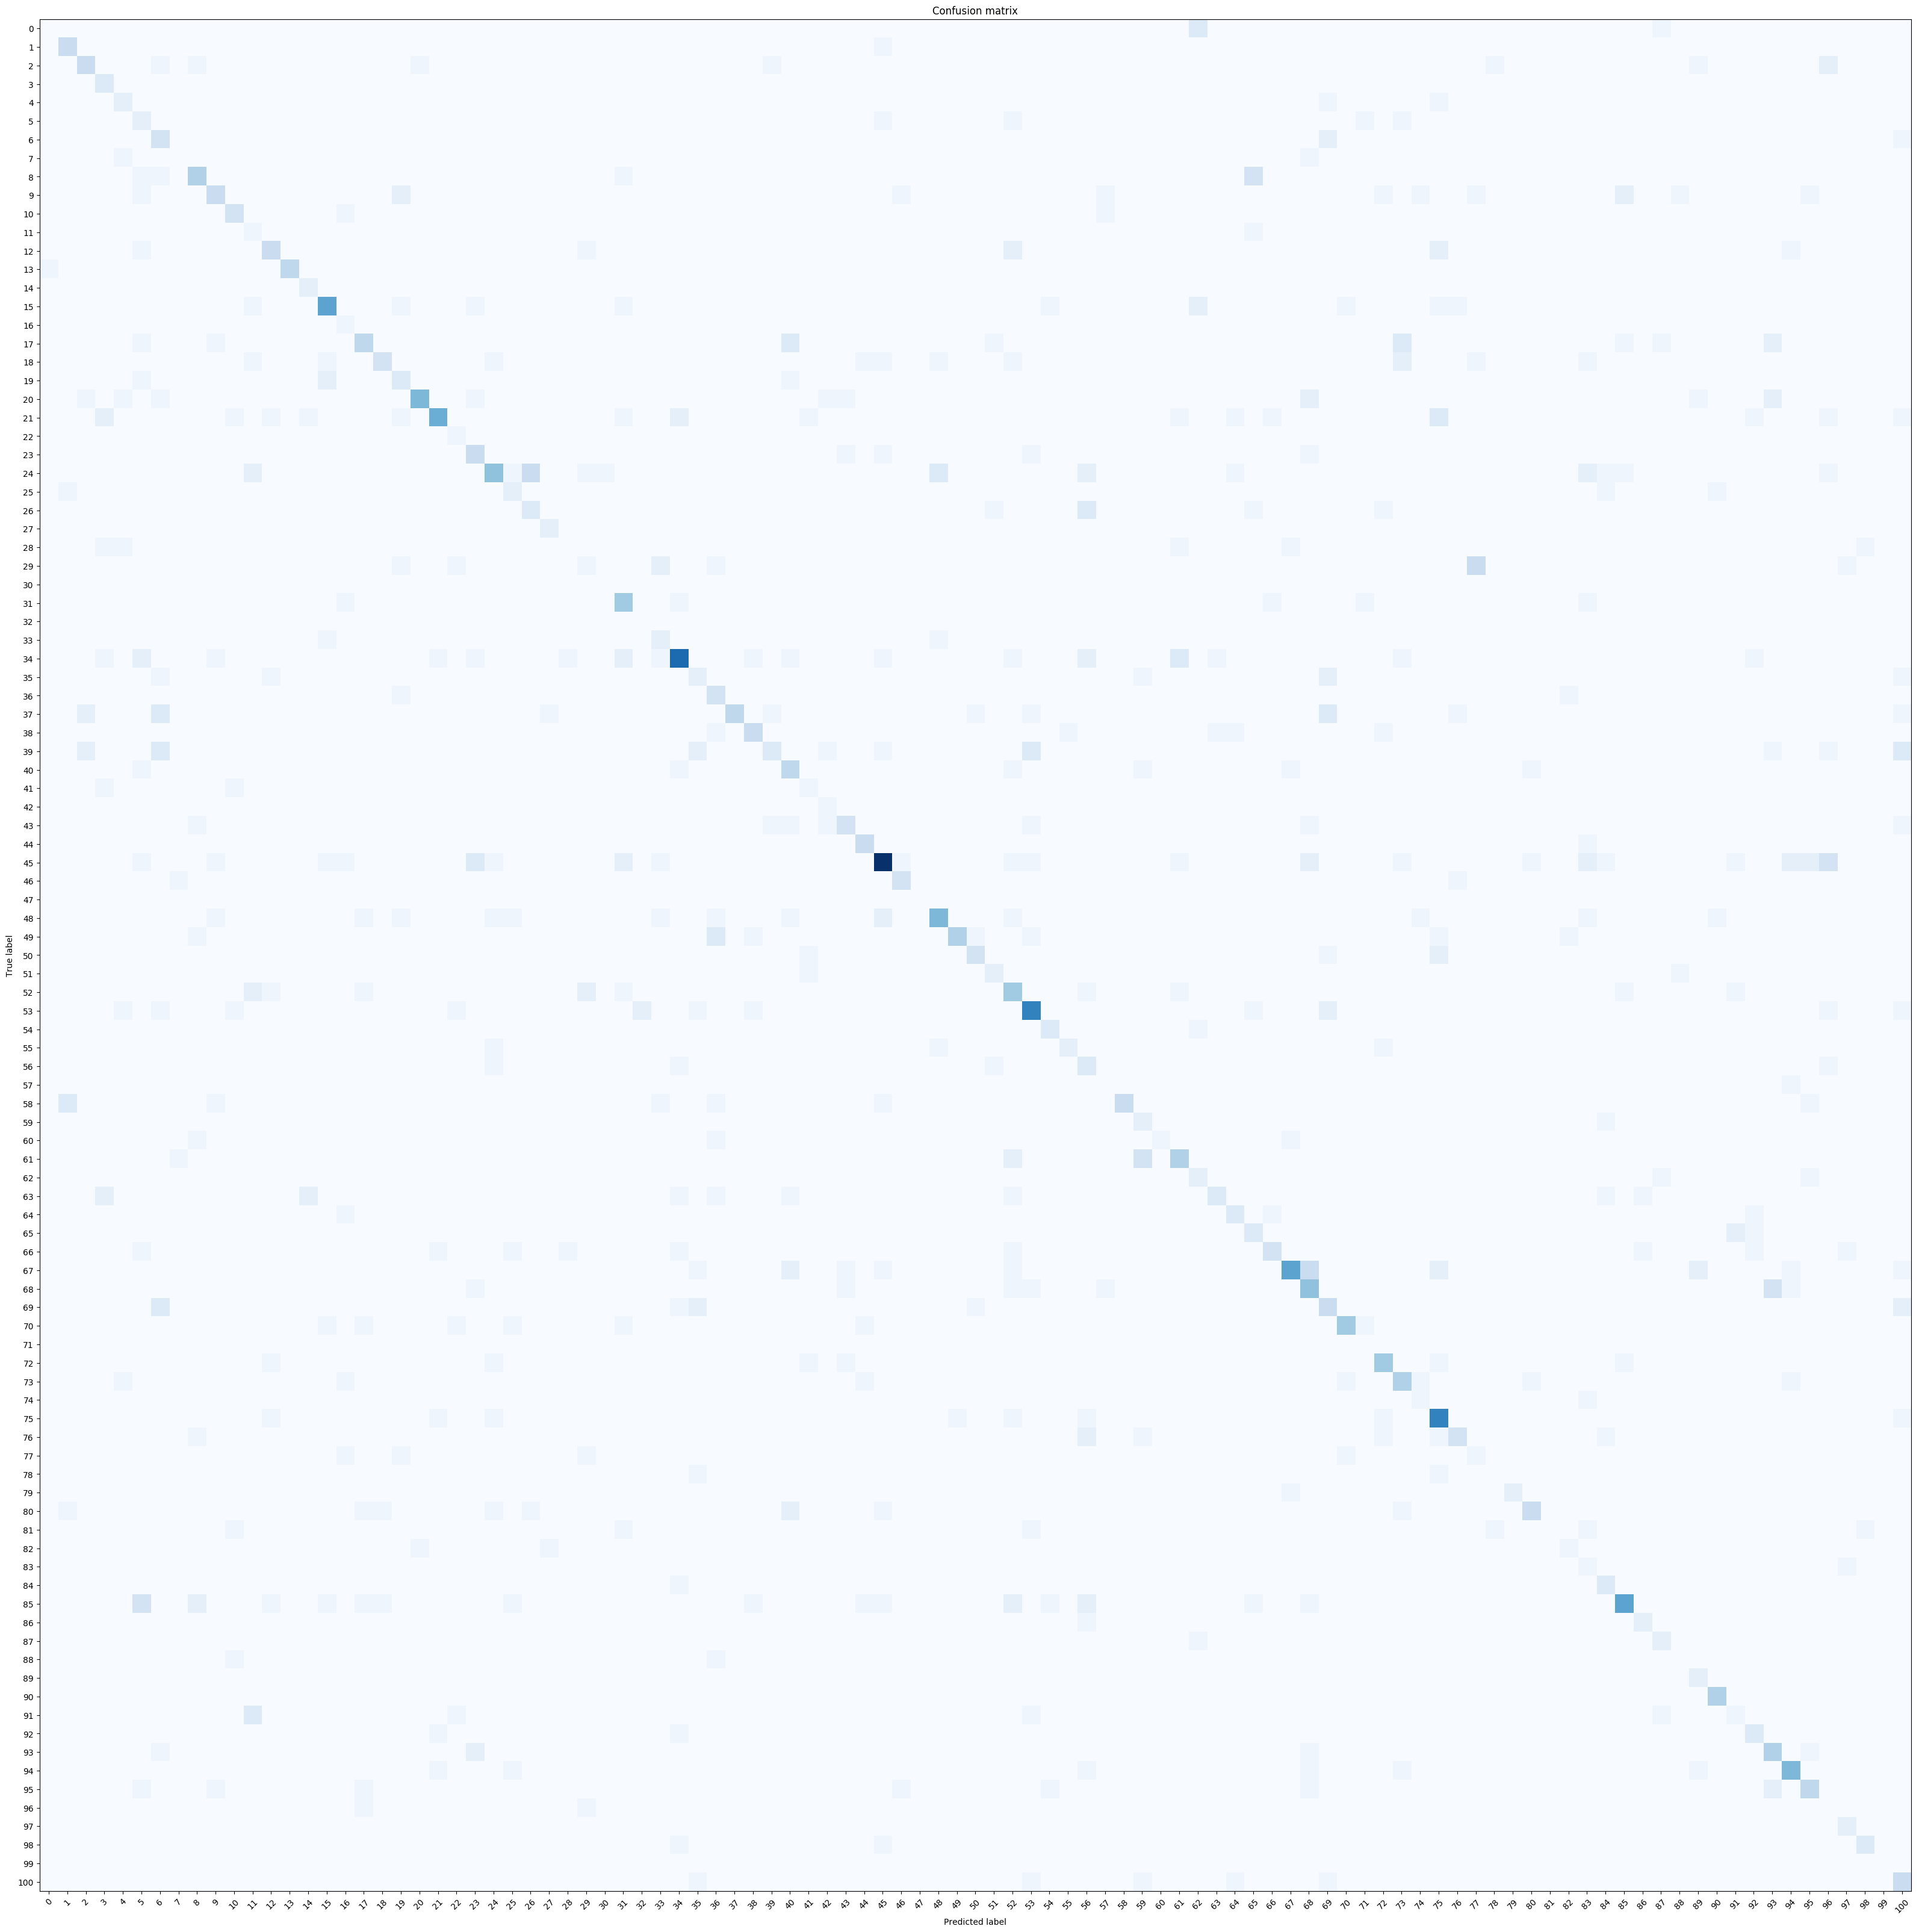
\includegraphics[width=\textwidth]{./fig/conf_mat_cnn_knn.png}
        \caption{Confusion matrix of targeted attacks using untargeted model}
        \label{fig:conf_mat_cnn_knn}
    \end{subfigure}
    \qquad
    \begin{subfigure}[b]{0.4\textwidth}
        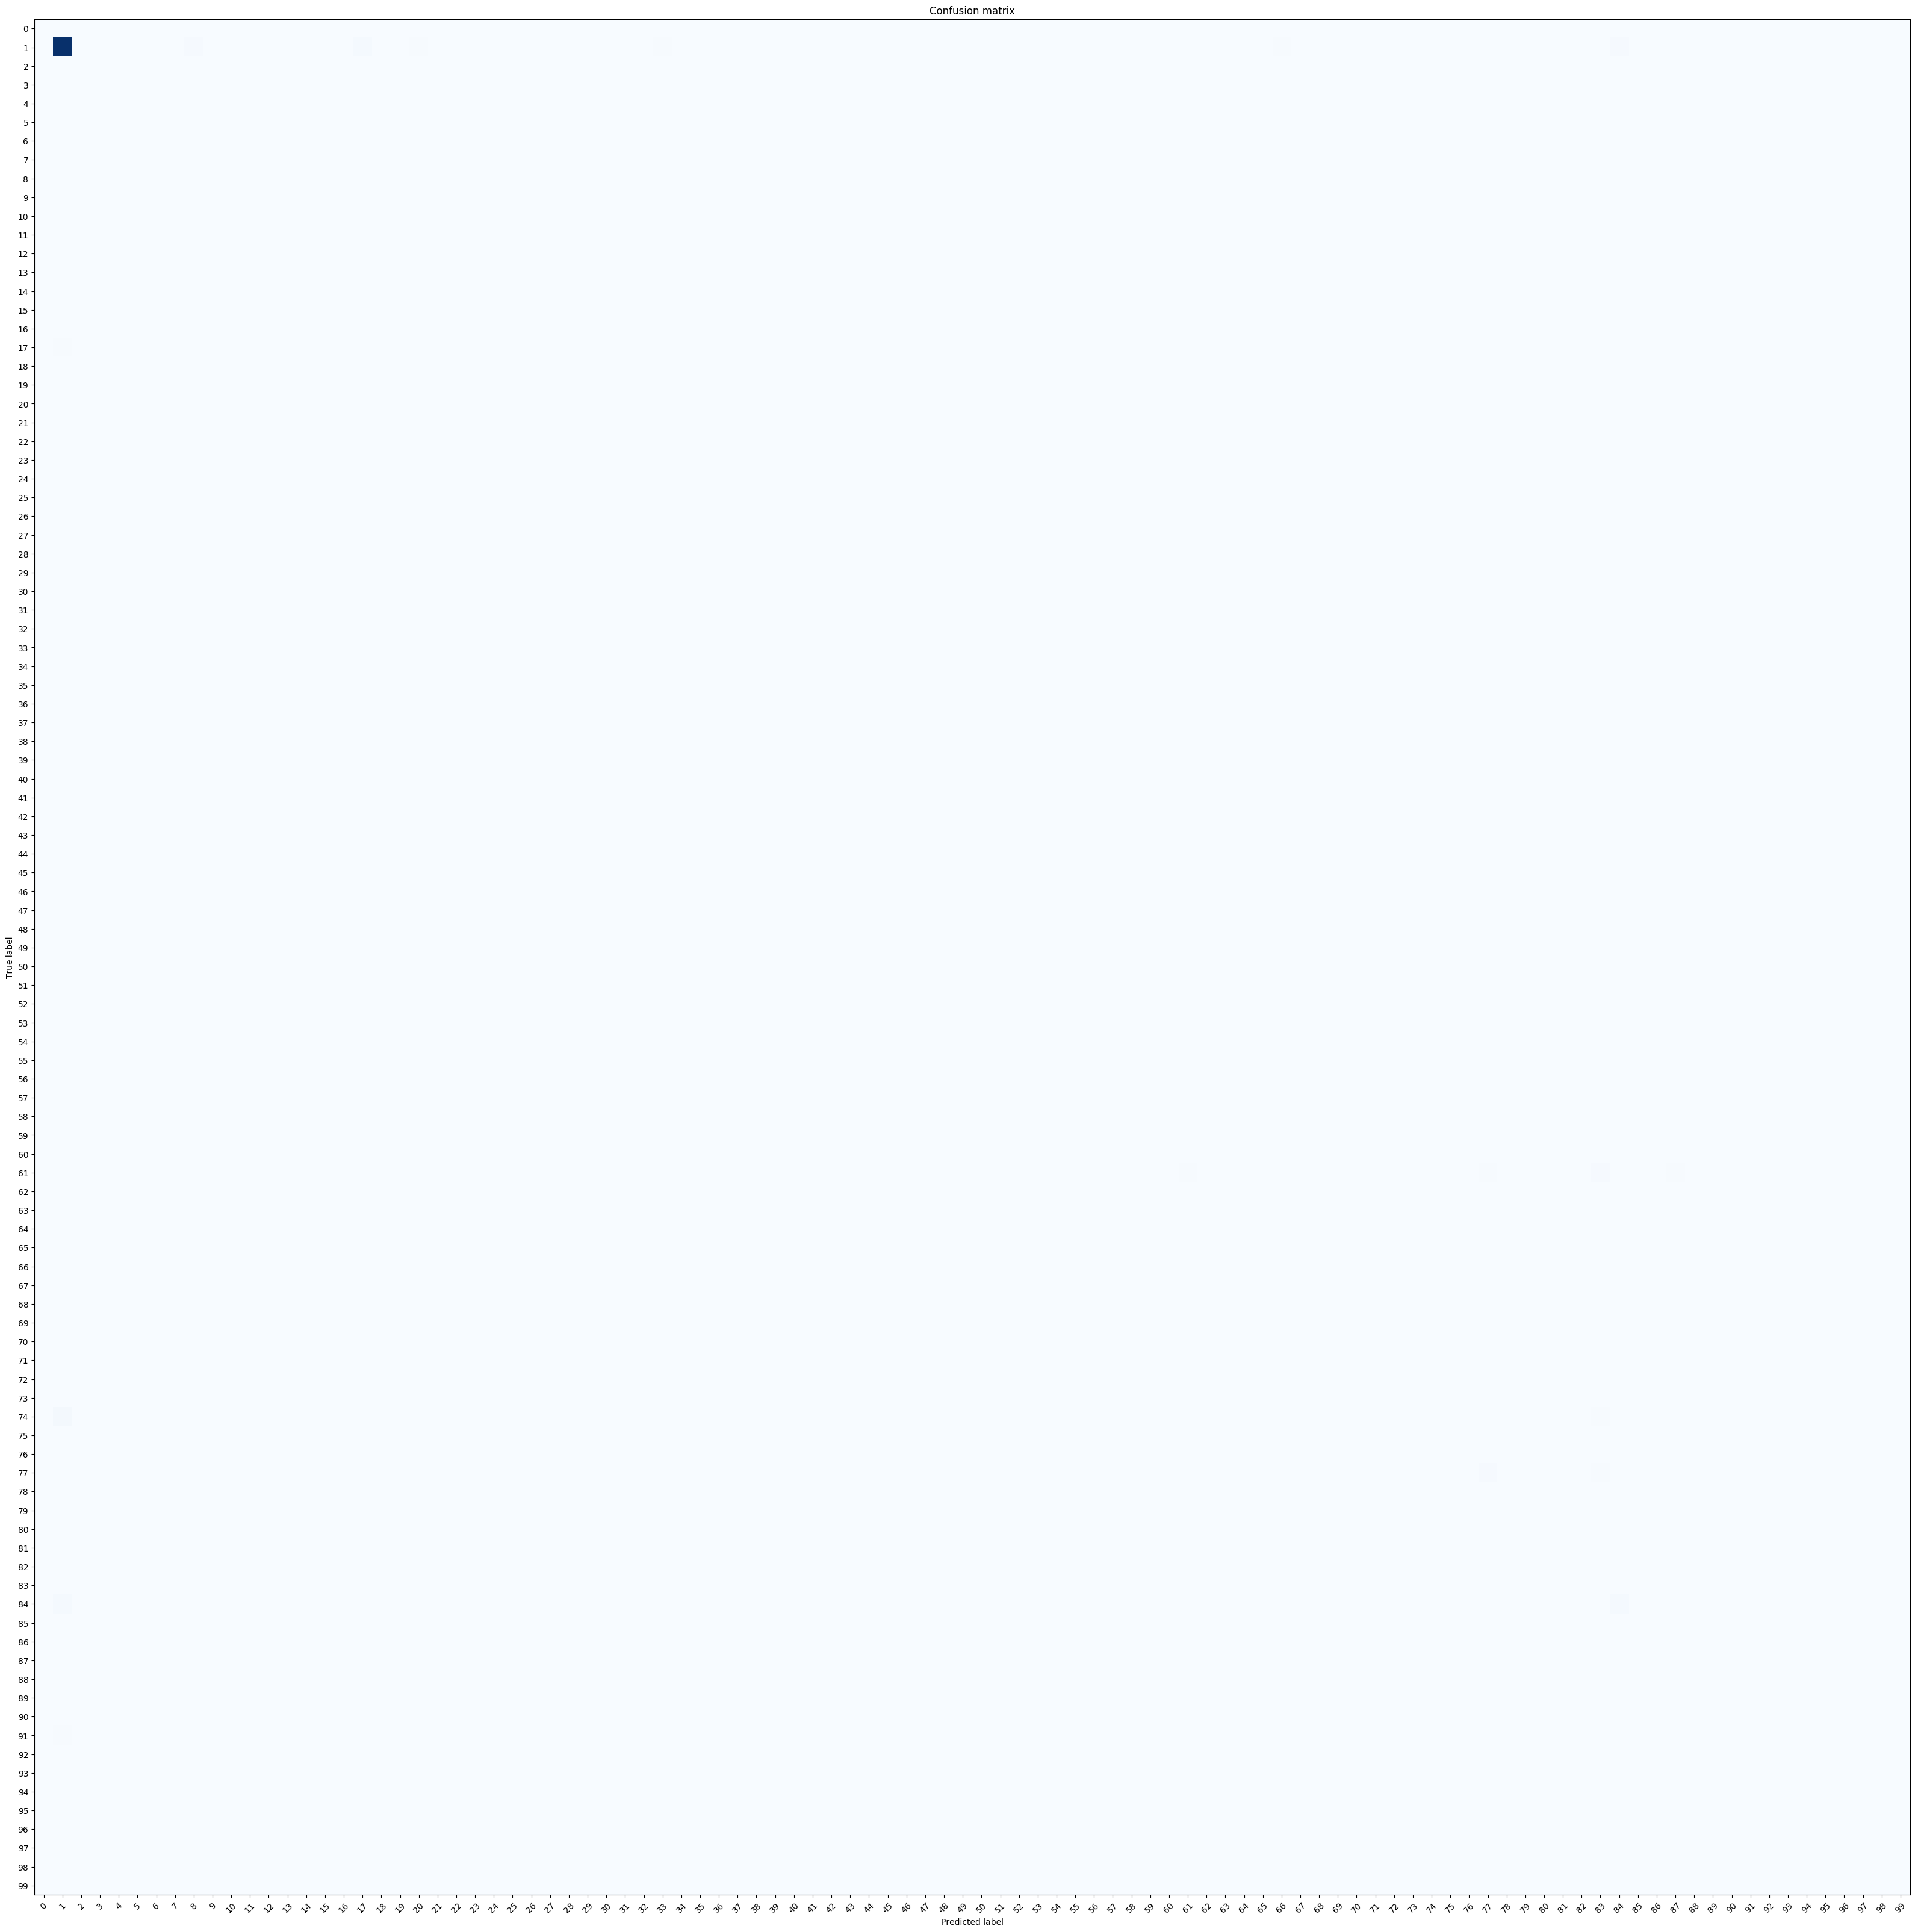
\includegraphics[width=\textwidth]{./fig/conf_mat_cnn_knn_targeted.png}
        \caption{Confusion matrix of targeted attacks using targeted model}
        \label{fig:conf_mat_cnn}
    \end{subfigure}
    \caption{Confusion matrix of targeted attacks}
    \label{fig:confusion_matrices}
\end{figure}
